\documentclass[11pt]{article}
\usepackage{ctex}
\usepackage[english]{babel}
\usepackage{blindtext}
\usepackage{nameref}
\usepackage{fancyhdr}
\usepackage{tabularx}
\usepackage{amsmath,amssymb,amsthm}
\usepackage{graphicx,float}
\usepackage{physics}
\usepackage{pgfplots}
\usepackage[a4paper, total={6in, 9in}]{geometry}
\usepackage{wrapfig}

\graphicspath{{../images/}}

\pagestyle{fancy}
\fancyhf{}
\fancyhf[HL]{Pre F4 Diagnose}
\fancyhf[CF]{\thepage}

\newcommand{\innerprod}[2]{\langle{#1},{#2}\rangle}
\newcommand{\id}{\mathtt{id}}

\newtheorem*{definition}{Definition}
\newtheorem*{theorem}{Theorem}
\newtheorem*{corollary}{Corollary}
\newtheorem*{lemma}{Lemma}
\newtheorem*{proposition}{Proposition}
\newtheorem*{remark}{Remark}
\newtheorem*{claim}{Claim}
\newtheorem*{example}{Example}
\newtheorem*{axiom}{Axiom}

\begin{document}
    \thispagestyle{plain}

    \centering 

    \section*{F4 Diagnostic Test\\MATHEMATICS Compulsory Part\\Question Paper}

    \raggedright

    \subsection*{Instructions}

    \begin{enumerate}
        \item This paper must be answered in English.
        \item Unless otherwise specified, all working must be clearly shown.
        \item Unless otherwise specified, numerical answers must be exact.
        \item This paper is for \textbf{internal use} only.
    \end{enumerate}

    \newpage

    \begin{enumerate}
        \item This is a simple algebra question. Solve the following system of linear equations:\begin{align*}
                \begin{cases}
                    2x+3y-5=0\\3x-2y+1=0
                \end{cases}
            \end{align*}
        \item This is a simple algebra question.\begin{enumerate}
            \item Make $y$ the subject of $\dfrac{x}{y}=\dfrac{\sqrt{y-7x-8}}{3y}$.
            \item Suppose $f(y)=y^2+2y$ and $y$ satisfy the equation in (a) with $y\neq 0$. Write $g(x)=f(y)$ when $y$ is being substituted by the corresponding formula in $x$. Factorize $g(x)$ in terms of $x$.
        \end{enumerate}
        \item This is some basic geometry.\begin{figure}[H]
            \centering
            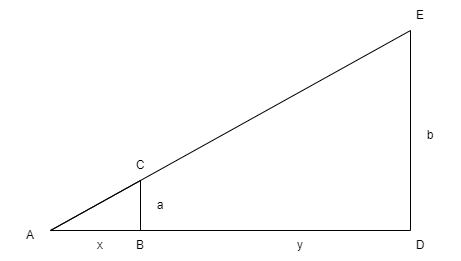
\includegraphics[scale=0.6]{similar_triangle.png}
        \end{figure}Given the above figure. $ACE$ and $ABD$ are straight lines and $\angle ABC=\angle ADE=90^\circ$. Also known that $AB=x$, $BD=y$, $BC=a$ and $DE=b$.\begin{enumerate}
            \item Prove that $\triangle ABC\sim\triangle ADE$.
            \item If $\angle CAB = 30^\circ$, with $b=10$ and $y=7\sqrt{3}$, find the area of $\triangle ABC$.
        \end{enumerate}
        \item Find the mean, mode, median of the following data: $$12,13,13,13,14,14,15,15,15,17,17,18$$

        \newpage
        \item Given a shooting board as following:\begin{figure}[H]
            \centering
            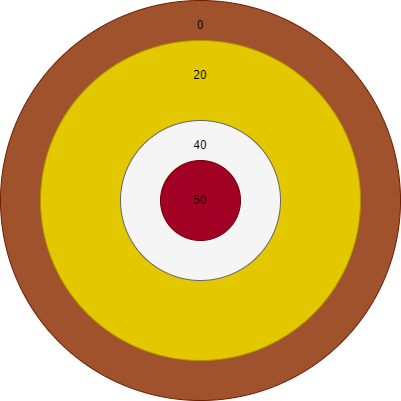
\includegraphics[scale=0.6]{shooting_board.png}
        \end{figure} It is given that the red zone is a circle of radius 5 cm, the white zone is a path of width 5 cm, the yellow zone is a path of width 10 cm, and the orange zone is a path of width 5 cm. Each zone owes the value written on the board. Suppose Owen is a shooter who has never missed any shots.\begin{enumerate}
            \item Find the probability for Owen to hit the red zone, the white zone, the yellow zone and the orange zone respectively. You may assume the chance of hitting every position on the board is equal. 
        \end{enumerate}
    \end{enumerate}

\end{document}